\documentclass[10pt,landscape]{article}
\usepackage[utf8]{inputenc}
\usepackage[left=0.25in,right=0.25in,top=0.25in,bottom=0.5in,a4paper, landscape]{geometry}
\setlength{\parindent}{0pt}
\setlength{\parskip}{0pt plus 0.5ex}
\usepackage[x11names]{xcolor} 
% \linespread{1.15} % Line spacing.


% Title sec:
% ==========

\usepackage{titlesec} % !Incompatible with beamer.
\titlelabel{\thetitle.\quad} % Dot after counter
\titleformat*{\section}{\Large\bfseries\color{Firebrick4}}
\titleformat*{\subsection}{\large\bfseries\color{Blue4}}
\titleformat*{\subsubsection}{\normalsize\bfseries\center}
\titlespacing*{\section}{0mm}{1ex plus 0.2ex minus 0.2ex}{0.5ex plus .1ex}
\titlespacing*{\subsection}{0mm}{1ex plus 0.2ex minus 0.2ex}{0.5ex plus .1ex}
\titlespacing*{\subsubsection}{0mm}{1ex plus 0.2ex minus 0.2ex}{0.5ex plus .1ex}
\setcounter{secnumdepth}{2}


% Mathematics:
% ============

\usepackage{amssymb,amsmath,amsthm,amsfonts}
\usepackage{centernot}
\usepackage{mathtools}
\usepackage{mathrsfs}

\everymath{\displaystyle} % Keeps same font size for inline math. For eg. in fractions.


\newtheoremstyle{mythmstl}{}{}{\itshape}{}{\bfseries}{:}{\newline}{\thmname{#1}\thmnumber{ #2}\thmnote{ (#3)}}%
\theoremstyle{mythmstl}
\newtheorem{theorem}{Theorem}[section]
\theoremstyle{plain} % default
\newtheorem{corollary}{Corollary}[theorem]
\newtheorem{lemma}[theorem]{Lemma}
\newtheorem{proposition}{Proposition}

\newtheoremstyle{mydefstl}{}{}{}{}{\bfseries}{:}{\newline}{\thmname{#1}\thmnumber{ #2}\thmnote{ (#3)}}%
\theoremstyle{mydefstl}
\newtheorem{definition}{Definition}[section]
\newtheorem{example}{Example}[section]
\newtheorem{exercise}{Exercise}[section]

\theoremstyle{remark}
\newtheorem*{remark}{Remark}
\newtheorem*{note}{Note}
\newtheorem*{case}{Case}


% New declarations
% ================
\usepackage{mathtools}
\DeclarePairedDelimiter\ceil{\lceil}{\rceil}
\DeclarePairedDelimiter\floor{\lfloor}{\rfloor}
\DeclarePairedDelimiter\angbrac{\langle}{\rangle}


% Tables and Box:
%================
\usepackage{tabularx} % To use table that wrap text and fit the column width.
\usepackage{multicol,multirow}
\usepackage{booktabs} % Necessary for \toprule \midrule in tables.
\usepackage{tabu} % Better tables.
\usepackage[framemethod=TikZ]{mdframed} % To make text boxes.


% URL
%========
\usepackage{url} % For \url{} Alternate for above.
\usepackage[colorlinks]{hyperref}
% USAGE: \href{url}{alias}
\hypersetup{citecolor=pink}
\hypersetup{linkcolor=red}
\hypersetup{urlcolor=blue}


% Others:
%========
\usepackage{enumitem}
\usepackage[os=win]{menukeys} % To use text in box that looks like keyboard keys.

\begin{document}

\raggedright
\footnotesize
\begin{multicols*}{3}
\setlength{\premulticols}{1pt}
\setlength{\postmulticols}{1pt}
\setlength{\multicolsep}{1pt}
\setlength{\columnsep}{2pt}


%%%%%%%%%%%%%%%%%%%%%%%%%%%%%%%%%%%%%%%%%%%%%%%%%%%%%%%%%%%%%%%%%%%%%%%%%%%%%%%%%%%%%%%%%%%%%%%%%%

\begin{center}
\begin{tabular}{c}
\Large{\textbf{The C++ programming language}}\\
\today\\
Ramasamy Kandasamy\\
\end{tabular}
\end{center}

%%%%%%%%%%%%%%%%%%%%%%%%%%%%%%%%%%%%%%%%%%%%%%%%%%%%%%%%%%%%%%%%%%%%%%%%%%%%%%%%%%%%%%%%%%%%%%%%%%

\section{Compile and Debug}

\subsection{G++}
Usage:\\
\texttt{g++ \textit{option} hello.cpp -o hello}\\
\texttt{g++ hello.cpp -o hello}\\
\texttt{g++ -O3 hello.cpp -o hello}\\
Options:\\
\begin{tabularx}{\linewidth}{lX}
\texttt{-o} & Output file name.\\
\texttt{-I} & Include additional directories in the search path. Eg:\\
& \texttt{g++ -I /home/user/libs foo.cpp}\\
\texttt{-O\textit{<level>}} & Optimization level, starts from 0. Eg: \texttt{-O3}\\
\texttt{-g} & Creates breakpoints for debugging using GDB.\\
\texttt{-lm} & Missing link. Used to link certain libraries like \texttt{math.h}.\\
\texttt{-E} & Output preprocessed but uncompiled code.\\
\texttt{-S} & Compile but do not assemble.\\
\texttt{-c} & Compile and assembly, but do not link.\\
\end{tabularx}

\subsection{GDB}
To run: \texttt{gdb hello}\\
\begin{tabularx}{\linewidth}{lX}
\texttt{break} & Set break point. Eg: \texttt{break \textit{function}} or \texttt{break \textit{line number}}.\\
\texttt{run} & Run the program. The program stops at every break point.\\
\texttt{next} & Run until next breakpoint.\\
\texttt{print} & Eg: \texttt{print i} or \texttt{print \&i}\\
\texttt{sizeof} & Eg: \texttt{print sizeof(i)}\\
\texttt{\&i} & Address of i.\\
\texttt{*j} & Content of memory location j.\\
\texttt{ptype} & get type of a variable. Eg: \texttt{ptype(i)}\\
\texttt{set var} & Reassign variable. Eg: \texttt{set var i = 1}\\
\texttt{disassemble} & Use after break and run. Gives assembly code.\\
\end{tabularx}

\textbf{Accessing memory location using x}\\
Usage: \texttt{x/nfs}. \texttt{nfs} describes the format.\\
n - Number of units to display.\\
f - Number format.\\
s - Size of each unit.\\
\begin{tabularx}{\linewidth}{lX}
\hline
\texttt{x} & Hex.\\
\texttt{o} & Octal.\\
\texttt{t} & Binary.\\
\texttt{d} & Decimal.\\
\texttt{u} & Unsigned decimal.\\
\texttt{i} & Instruction.\\
\texttt{c} & Character.\\
\texttt{s} & String.\\
\hline
\texttt{b} & byte.\\
\texttt{h} & Halfword.\\
\texttt{w} & Word.\\
\texttt{g} & Giant.\\
\hline
\end{tabularx}



\vfill\null
\columnbreak

\section{Pre-processor directives}

\begin{minipage}{\linewidth}
Pre-processor directive always start with a '\texttt{\#}'.

\begin{itemize}
    \item \texttt{\#include \textit{filename}}\\
    Replace with contents of \textit{filename}\\

    \begin{itemize}
        \item files with double quotes: \texttt{\# include "file.h"}\\
            First pre-processor looks for \texttt{file.h} in the same directory as the source file and then in pre-configured list of standard system directories.
        \item files with angle bracket: \texttt{\# include <stdio.h>}\\
            The pre-processor looks only in the pre-configured list of standard system directories.
        \item Additional directories can be include
    \end{itemize}
\end{itemize}

\begin{itemize}

    \item \texttt{\#define NAME \textit{replacement text}} \\
    \texttt{NAME} is replaced with \texttt{\textit{replacement text}} \\
    \item \texttt{\#define \textit{token}(arg1,arg2) \textit{statement}} \\
    Defining a macro. Eg: \\
    \texttt{\#define max(A,B) ((A) > (B) ? (A) : (B))}
    \item \texttt{\#undef NAME} \\
    Nullifies existing definition of \texttt{NAME}. Used to ensure a routine is a function.\\
    \item \texttt{\#if}, \texttt{\#elif},\texttt{\#else}, \texttt{\#endif}\\
    Eg-1:\\
    \texttt{\#if !define(HDR)}\\
    \texttt{\#define HDR}\\
    \texttt{/*contents of hrd.h*/}\\
    \texttt{\#endif}\\
    NOTE: \texttt{define()} after \texttt{\#if} returns \texttt{1} if its argument is already defined.\\ 
    Here \texttt{\#define HDR} is first line of \texttt{hrd.h} and this file is included only if it was not already included.
    Eg-2:\\
    \texttt{\#if SYSTEM == SYSV }\\
    \qquad \texttt{\#define HDR "sysv.h"}\\
    \texttt{\#elif SYSTEM == BSD}\\
    \qquad \texttt{\#define HDR "bsd.h"}\\
    \texttt{\#elif SYSTEM == MSDOS}\\
    \qquad \texttt{\#define HDR "msdos.h"}\\
    \texttt{\#else}\\
    \qquad \texttt{\#define HDR "default.h"}\\
    \texttt{\#endif}\\
    \item \texttt{\#ifdef}  and \texttt{\#ifndef}\\
    Test whether a name is already defined.\\
    Eg-1 in above point can be replaced by:
    \texttt{\#ifndef HDR}\\
    \texttt{\#define HDR}\\
    \texttt{/*contents of hdr.h*/ }\\
    \texttt{\#endif}\\
\end{itemize}
\end{minipage}

\vfill\null
\columnbreak

% \section{Memory layout of Cpp program}
Adapted from\\
\url{https://www.geeksforgeeks.org/memory-layout-of-c-program/}\\
\vspace{5pt}

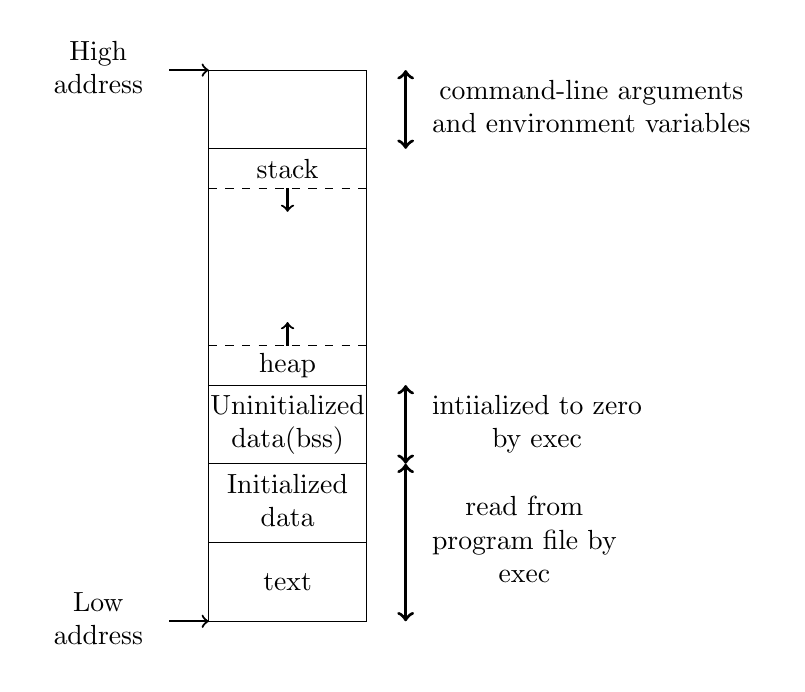
\begin{tikzpicture}
	\draw (0,0) rectangle (2,7);
	\draw [->, thick] (-0.5, 0) -- (0,0);
	\draw [->, thick] (-0.5, 7) -- (0,7);
	\draw (0, 1) -- (2, 1);
	\draw (0, 2) -- (2, 2);
	\draw (0, 3) -- (2, 3);
	\draw [dashed] (0, 3.5) -- (2, 3.5);
	\draw [->, thick] (1,3.5) -- (1,3.8);
	\draw [dashed] (0, 5.5) -- (2, 5.5);
	\draw [->, thick] (1,5.5) -- (1,5.2);
	\draw (0,6) -- (2,6);
	\draw [<->, very thick] (2.5, 6) -- (2.5, 7);
	\draw [<->, very thick] (2.5, 0) -- (2.5, 2);
	\draw [<->, very thick] (2.5, 2) -- (2.5, 3);
	\node at (1, 0.5) {text}; 
	\node at (1, 1.5) {\begin{tabular}{c}Initialized\\data\end{tabular}}; 
	\node at (1, 2.5) {\begin{tabular}{c}Uninitialized\\data(bss)\end{tabular}}; 
	\node at (1, 3.25) {heap};
	\node at (1, 5.75) {stack};
	\node at (-0.5, 0) [anchor = east] {\begin{tabular}{c} Low\\address \end{tabular}};
	\node at (-0.5, 7) [anchor = east] {\begin{tabular}{c} High\\address \end{tabular}};
	\node at (2.5, 6.5) [anchor = west] {\begin{tabular}{c} command-line arguments\\ and environment variables \end{tabular}};
	\node at (2.5, 1) [anchor = west] {\begin{tabular}{c} read from \\ program file by \\ exec \end{tabular}};
	\node at (2.5, 2.5) [anchor = west] {\begin{tabular}{c} intiialized to zero \\ by exec \end{tabular}};
\end{tikzpicture}

In linux the command \texttt{size} can be used to see memory allocation of a compiled C program.\\
Eg: 
 
\begin{mdframed}
	\texttt{\$ size a.out}\\
	\texttt{    text	   data	    bss	    dec	    hex	filename}\\
	\texttt{   1525	    600	      8	   2133	    855	}\\
\end{mdframed}

\textcolor{red}{Where is heap and stack located physically ?}\\
See:\\
\url{https://stackoverflow.com/questions/79923/what-and-where-are-the-stack-and-heap}

\begin{tabularx}{\linewidth}{l|X}
	
\end{tabularx}


\vfill \null
\columnbreak



\section{Variables and Constants}

\subsection{Variable types}
\begin{tabularx}{\linewidth}{lllX}
Type & Location & memory location & Scope\\
\hline
\texttt{Global} & Outside functions & data/bss & Global\\
\texttt{Static} & Outside functions & data/bss & Source file\\
\texttt{Static} & Inside a function & data/bss & Local\\
\texttt{Local} & Inside a function & stack & Local\\
\texttt{Register$^\#$} & Inside a function$^*$ & register & Local\\
\hline
\end{tabularx}
$^*$ causes error if declared in global space.\\
$^\#$ This is not strict. The compiler might choose not to keep the variable in register.

\subsection{Variable declaration and initialization}
\begin{itemize}
\item Eg: \texttt{int num;}
Local or global depending on context.
\item Eg: \texttt{static int num;}
Static variable.
\item Eg: \texttt{const int num;}
Causes error if \texttt{num} is modified.
\end{itemize}
\subsection{Data types}
\textbf{Major variable types}
\begin{tabularx}{\linewidth}{lX}
\texttt{char} & 1 byte.\\
\texttt{short int} & 2 bytes.\\
\texttt{int} & 4 bytes.\\
\texttt{long int} & 4 to 8 bytes.\\
\texttt{long long int} & 8 bytes.\\
\texttt{\_\_int128\_t} & 16 bytes, not part of standard definition, but is supported by g++.\\ 
\texttt{float} & 4 bytes.\\
\texttt{double} & 8 bytes.\\
\texttt{long double} & 80 bit floating point supported by g++.\\
\texttt{size\_t} & unsigned type.\\
\end{tabularx}
Their actual size might vary depending on the system.\\

\textbf{Modifiers for variable types}
\begin{tabularx}{\linewidth}{lX}
\texttt{unsigned} & With int and char.\\
\texttt{signed} & With int and char.\\
\end{tabularx}


\subsection{Constants}

\begin{tabularx}{\linewidth}{lX}
\texttt{1234} & \texttt{int}\\
\texttt{1234567890L} & \texttt{long int}. \textcolor{red}{When should I use L?}\\
\texttt{010} & Octal $\equiv$ 8.\\
\texttt{0x10} & Hexadecimal $\equiv$ 16.\\
\texttt{0b10} & Binary $\equiv$ 2. Binary format is not part of standard C, but is supported by gcc.\\
'x' & Character constant, has an integer value.\\
'\textbackslash ooo' & Specify ASCII code of the character in octal.\\
'\textbackslash xhh' & Specify ASCII code of the character in hexadecimal.\\
\end{tabularx}

\textbf{Escape sequences:}\\
 \texttt{\textbackslash a, \textbackslash b, \textbackslash f, \textbackslash n, \textbackslash r, \textbackslash t, \textbackslash v, \textbackslash \textbackslash, \textbackslash ?, \textbackslash ', \textbackslash "}.

\textbf{Enumeration constants}: List of constant integers.\\

\begin{itemize}
\item Eg: \texttt{enum ans \{NO, YES\};}\\
By defaults integers are assigned from 0.
\item Eg: \texttt{enum days \{MON=1,TUE,WED,THU,FRI,SAT,SUN\};}\\
Here, \texttt{MON} is assigned 1, and by default, \texttt{TUE} is 2. 
\item Eg: \texttt{enum months \{JAN =1, FEB, APR=4,MAY\};}\\
Here, \texttt{MAY} is 5.
\end{itemize}


\section{Arithemetic and logical operation}

    \begin{tabularx}{\linewidth}{l|lX}
        \hline\\
        & Operators & Associativity \\
        \hline \\
        1 & \texttt{() [] -$>$} \textbf{.} & left to right\\
        2 & \texttt{! $\tilde{}$ ++ -- + - * \& (type) sizeof} & right to left\\
        3 & \texttt{* / \%}(reminder) & left to right\\
        4 & \texttt{+ -} & left to right \\
        5 & \texttt{$<<$ $>>$} & left to right \\
        6 & \texttt{$<$ $<=$ $>$ $>=$}  & left to right\\
        7 & \texttt{== !=} & left to right\\
        8 & \texttt{\&} & left to right \\
        9 & \texttt{\^} & left to right \\
        10 & \texttt{|} & left to right\\
        11 & \texttt{\&\&} & left to right\\
        12 & \texttt{||} & left to right \\
        13 & \texttt{?:} & left to right \\
        14 & \texttt{= += -= *= /= \%= \&= \^{}= |= $<<$= $>>$=} & right to left\\
        15 & \texttt{,} & left to right\\
        \hline
    \end{tabularx}

    \subsection{Explanation for selected operators}

        \begin{itemize}
            \item \texttt{->} and \textbf{.}\\
            See \textbf{Structures}.
            \item \textbf{Casting}\\
            Changes the type of a variable.\\
            Eg:  \texttt{float a = (int) 3/2;}// \texttt{a} is 1.0.\\
            \item \textbf{sizeof}\\
            \texttt{sizeof num;} // Give size of the variable num.\\
            \texttt{sizeof (int)} // Gives size of int, i.e. 4.\\
            \item \textbf{Bitwise operators}
            \begin{itemize}
            \item \texttt{>>}\\
            Eg: \texttt{a = b >> 1} //Shift \texttt{b} bitwise to the right by 1 bit.\\
            Fill left most bits with the original left most bit.
            \item \texttt{<<}\\
            Eg: \texttt{a = b << n} //Shift \texttt{b} bitwise to the left by n bits.\\
            Fill right most bits with zero.
        \end{itemize}

        Others:\\
        \begin{tabularx}{\linewidth}{l|X}
            \hline
            \texttt{\&} & Bitwise AND\\
            \texttt{$\mid$} & Bitwise inclusive OR\\
            \texttt{\^} & Bitwise EXOR\\
            \texttt{\~} & Bitwise NOT\\
            \hline
        \end{tabularx}


        \item \textbf{Comma operator}
        \begin{itemize}
            \item \texttt{expr1,expr2}\\
            Use sparingly, Eg: \texttt{i++,j--}\\
            \item \texttt{x = (Conditional expresion)? \textit{expr1}: \textit{expr2}}\\
            \texttt{x =expr1} if \texttt{Conditional expression} is true, else \texttt{x = expr2}.
        \end{itemize}

        \end{itemize}



\section{Control Flow }

\begin{minipage}{\linewidth}

\begin{tabularx}{\linewidth}{l|X}
    \hline\\
    \textbf{If-else} & \texttt{if (\textit{expression})} \\ &
    \texttt{\qquad \textit{statement}} \\ &
    \texttt{else if (\textit{expression})} \\ &
    \texttt{\qquad \textit{statement}} \\ &
    $\vdots$\\ &
    \texttt{else} \\ &
    \texttt{\qquad \textit{statement}}\\

    \hline

    \textbf{Switch} & \texttt{switch (\textit{expression})}\\
    & \texttt{\{}\\
    & \texttt{\qquad case \textit{const-expr}: \textit{statements}; break;}\\
    & \texttt{\qquad case \textit{const-expr}: \textit{statements}; break;}\\
    & \texttt{\qquad default: \textit{statements}; break;} \\
    & \texttt{\}}\\

    & Without break statement the execution will \textit{fall through} all the cases.\\
    & \texttt{This can be used as:} \\
    %
    & \texttt{switch (\textit{expression})}\\
    & \texttt{\{} \\
    & \hspace{10pt} \\
    & \texttt{\qquad case 1: case 2: case 3:}\\
    & \texttt{\qquad \qquad group = 0;}\\
    & \texttt{\qquad \qquad break;}\\
    & \texttt{\qquad case 4: case 5:}\\
    & \texttt{\qquad \qquad group = 1;}\\
    & \texttt{\qquad \qquad break;}\\
    & \texttt{\qquad default:} \\
    & \texttt{\qquad \qquad group = -1;}\\
    & \texttt{\qquad \qquad break;}\\
    & \texttt{\}}\\
    \hline\\
    \textbf{While} & \texttt{while (\textit{expression})}\\
    & \texttt{\qquad \textit{statement}}\\
    \hline \\
    \textbf{For} & \texttt{for (expr1; expr2; expr3)}\\
    & \texttt{\qquad \textit{statement}} \\
    & This for loop is equivalent to:\\
    & \texttt{expr1;}\\
    & \texttt{while (expr2)} \\
    & \texttt{\{}\\
    & \texttt{\qquad statements;}\\
    & \texttt{\qquad expr3;}\\
    & \texttt{\{}\\
    \hline\\
    \textbf{Do While} & \texttt{do}\\
    & \texttt{\qquad \textit{statement}}\\
    & \texttt{while (\textit{expression});}\\
    \hline\\
    \textbf{Break} & \texttt{break} : Exit the the loop or control.\\
    & \texttt{Works for \texttt{while, for, do while} and \texttt{switch}}\\
    \hline
\end{tabularx}
\end{minipage}

\begin{minipage}{\linewidth}
\begin{tabularx}{\linewidth}{l|X}

    \textbf{Continue} & \texttt{continue}: Continue next iteration.\\
    & Works for \texttt{while, for, do while}\\
    & If \texttt{switch} is within a loop and if \texttt{continue} is used inside \texttt{switch} and if it is executed, then the loop skips to next loop.\\
    \hline\\

    \hline\\
    \textbf{Goto and label} & Example:\\
    & \texttt{if (disaster)}\\
    & \texttt{\{}\\
    & \texttt{\qquad goto error;}\\
    & \texttt{\}}\\
    & $\cdots$\\
    & \texttt{error:}\\
    & \texttt{\{}\\
    & \texttt{\qquad \textit{statement}}\\
    & \texttt{\}}\\
    \hline
\end{tabularx}

\begin{mdframed}[backgroundcolor=blue!20]
    \textbf{Shorter alternative for \texttt{if-else} statement:}

    \texttt{x = <cond-expr> ? <out-if-true> : <out-if-false>;}\\
    Eg: \texttt{char is\_pos = (n > 0) ? 'y' : 'n';}\\
\end{mdframed}

\end{minipage}

\vfill \null
\columnbreak


\section{Functions}

\subsection{\texttt{int main} function: command line arguments}

\texttt{main(int argc, char *argv[])}\\
\texttt{\{}\\
\qquad \texttt{$\cdots$}\\
\texttt{\}}

\begin{tabularx}{\linewidth}{l|X}
\texttt{argc} & Number of arguments including the program name. \\
\texttt{argv[0]} & Pointer to program name.\\
& \textcolor{red}{NOTE: \texttt{argv[0] represents name of the compiled program and not the source file and how it is called eg: \texttt{a.out} vs \texttt{./a.out}}}\\
\texttt{argv[i]} & Pointer to i$^{th}$ argument.\\
\texttt{argv[argc - 1]} & Pointer to last argument. \\
\end{tabularx}




\subsection{Function definition}
\texttt{\textit{type function\_name}(\textit{argument list})}\\
\texttt{\{}\\
\qquad \texttt{\textit{statements}}\\
\qquad \texttt{$ \cdots $}\\
\qquad \texttt{return \textit{expression}}\\
\texttt{\}}

eg:\\

\texttt{int foo(int num, int cars[],char *pn)}\\
\texttt{\{}\\
\qquad \texttt{\textit{statements}}\\
\qquad \texttt{$ \cdots $}\\
\qquad \texttt{return \textit{expression}}\\
\texttt{\}}

\subsection{Function declaration}

\textbf{Implicit declaration}:\\
The function is assumed to return \texttt{int}. Nothing is assumed about the arguments.\\
\textbf{Explicit declaration}:\\
Examples:\\
\texttt{int foo(int, int [], int *);}\\
\texttt{int foo(int x, int y[], int *p);}\\
Explicit declaration is not necessary if the function is defined before \texttt{main()}.\\

\subsection{Passing functions as arguments}
Example: passing \texttt{foo2} to \texttt{foo}.\\
\textbf{Declaration:}\\
\texttt{int foo(int x, int (*foo2)(int y));}\\
\textbf{Usage:}\\
\texttt{foo(x, foo2);}\\
\textcolor{red}{Also see:}\textit{7.7 Pointers to functions} 
\vfill \null
\columnbreak




\section{Pointers and arrays}

\subsection{Pointers}

\begin{tabularx}{\linewidth}{l|X}
\hline
Declaration & \texttt{\textit{type} *\textit{ptr};}\\
& Eg: \texttt{int *p;}\\
\hline
Initialization & \texttt{\textit{type *ptr = val};}\\
& Eg: \texttt{int *p = 0;}\\
& Eg: \texttt{int *p = NULL;}// Null pointer.\\
& Eg: \texttt{int *p = (int *) 100;}\\
& NOTE: Casting is required for integer other than zero. Also, the above memory location may not be available.\\
\hline
\texttt{\&} & Gives address.\\
& Eg: \texttt{ptr = \&x;}\\
\hline
\texttt{*} & Dereferencing operator.\\
& Eg, \texttt{*ptr} refers to x.\\
\hline
\end{tabularx}

\subsection{Arrays}

\begin{itemize}
\item \textbf{Character arrays}\\
\texttt{char s[100];}\\
\texttt{s = "abc";} //ERROR.\\
\texttt{*s = "abc";} // OK.\\
\texttt{char s[] = \{'a','b','c'\};}\\
\texttt{char s[] = "abc";}\\
\item \textbf{Integer, float arrays}\\
\texttt{int num[100]}\\
\texttt{num = \{1,2,3\}} // ERROR\\
\texttt{*num = \{1,2,3\}} // ERROR \\
\texttt{int num[] = \{1,2,3\}}\\
\texttt{float num[] = \{1.0,2.0,3.0\}}\\
\end{itemize}

\subsection{Character pointers}

\textbf{Examples:}\\

\texttt{char *pmessage;}\\
\texttt{pmessage = "Hello, World!\textbackslash n";} \\
\texttt{printf("\%s",pmessage); \# Prints the string}\\
\texttt{*pmessage} refer to '\texttt{H}'\\

\subsection{Pointer to pointers}

\textbf{Examples:}\\

\begin{tabularx}{\linewidth}{l|X}
\texttt{int **p} & \texttt{p} is a pointer to a pointer to \texttt{int}\\
& \texttt{*p} is poiner to a pointer to \texttt{int}\\
\texttt{char *line[MAXLEN]} & \texttt{line} is a pointer to a character array.\\

\end{tabularx}

\subsection{Multi-dimensional arrays}

I think, multi-dimensional arrays can be thought of as pointers to pointers etc.\\

Example:\\
Given: \texttt{int a[2][3] = \{\{1,2,3\},\{4,5,6\}\} } \\
The following are equivalent:\\

\begin{tabular}{l|l}
\hline
\texttt{a[0][0]} & \texttt{**a}\\
\hline
\texttt{a[1][1]} & \texttt{*(*(a + 1) + 1)}\\ 
\hline
\end{tabular}

\hspace{10pt}\\

Here \texttt{a} is a pointer to an array of pointers. 

\subsection{Arrays and pointers}
The following two are equivalent:\\

\begin{tabular}{l|l}
\hline
\texttt{pa = \&a[0];} & \texttt{pa = a;}\\
\texttt{a[i]} & \texttt{*(a + i)}\\
\texttt{p[i]} & \texttt{*(p + i)}\\
\texttt{f(int arr[])} & \texttt{f(int *arr)}\\
\hline
\end{tabular}

\begin{tabular}{l|l}
\hline
Legal & Illegal\\
\hline
\texttt{pa++} & \texttt{a++}\\
\texttt{pa[-1]} & \texttt{a[-1]}\\
\hline
\end{tabular}

\subsection{Pointer to functions}



Eg: \\
\texttt{int sum\_f(int size, int arr[], int (*foo)(int ))} // Definition.\\
\texttt{\{}\\
\qquad \texttt{int sum = 0;}\\
\qquad \texttt{for (int i = 0; i < size; i++)}\\
\qquad \qquad \texttt{sum += (*foo)(arr[i]);}\\
\texttt{\}}

Here \texttt{foo} is a pointer to a function and \texttt{(*foo)} is the function.\\

\texttt{sum\_f(size, arr, square)} // Usage.Sum of squares.\\
\texttt{sum\_f(size, arr, cube)} // Usage.Sum of cubes.\\

NOTE: Function names act as pointers to the function. \\


\vfill \null
\columnbreak



% Structures, unions and typedefs.
\section{Structures, unions and typedefs}

\subsection{Structure}

\begin{itemize}
\item \textbf{Definition:}\\
\texttt{struct point}\\
\texttt{\{}\\
\qquad \texttt{int x;}\\
\qquad \texttt{int y;}\\
\texttt{\};}\\

NOTE-1: Structure tag is optional??\\
NOTE-2: In C  a function cannot be a member of a structure.\\

\item \textbf{Declaration examples:}\\
\begin{itemize}
\item \texttt{struct \{$\cdots$\} a,b,c;}\\
\item \texttt{struct point \{$\cdots$\} a,b,c;}\\
\item \texttt{struct point a,b,c}\\
\item \texttt{struct point *p;}\\
\end{itemize}

\item \textbf{Accessing members}\\
\texttt{a.x = 5;}\\
\texttt{printf("\%d\textbackslash n",a.x);}\\

\item \textbf{Accessing members with pointer}\\
\texttt{struct point *p = \&a;}\\
The following are equivalent:\\
\begin{itemize}
\item \texttt{p -> x;}\\
\item \texttt{(*p).x;}\\
\item \texttt{a.x;}
\end{itemize}

\item \textbf{Arrays of structure:}\\
\texttt{struct points pts[100];}\\
\texttt{struct \{$\cdots$\} pts[] = \{\{$\cdots$\},\{$\cdots$\},$\cdots$,\{$\cdots$\}\};}\\
NOTE: In above assignment, in the RHS, elements within the braces could be of different types matching the members of the structure.\\
In case of simple members, each members need not be enclosed within braces.\\
 
\end{itemize}

\subsection{typedef}
end{itemize}
\begin{itemize}
	\item
		\texttt{typedef int Length;}\\
		\texttt{Length len, maxlen;}\\
		\texttt{Length *length[];}\\
		\texttt{typedef struct tnode *Treeptr;}\\
		\texttt{typedef struct tree Treenode;}\\
	\item The above examples could also be implemented by \texttt{\#define}\\
		The following can only be implemented by \texttt{typedef}:\\
		\texttt{typedef int (*PFI) (char*, char*);}
\end{itemize}

\subsection{Union}
A union is a variable that may hold objects of different types and sizes.\\
The syntax is based on structures:\\
\texttt{union u\_tag \{}\\
\texttt{\qquad int ival;}\\
\texttt{\qquad float fval;}\\
\texttt{\qquad char *sval;}\\
\texttt{\} u;}\\

For example, integer value of u can be accessed as:\\
\texttt{u.ival}

\subsection{Bit fields}

Eg:\\
\texttt{
	struct \{\\
		\qquad unsigned int is\_keyword : 1;\\
		\qquad unsigned int is\_extern : 1;\\
		\qquad unsigned int is\_static: 1;\\
	\} flags;
}\\

This defines \texttt{flags} that contains three 1-bit fields.\\
The number following the colon represents the field width.\\

\textbf{Namespace}
\texttt{using namespace std;}\\
	With this statement standard library functions can be used without the prefix \texttt{std::}\\


% Lambda functions.
\section{Lambda Functions}

\textit{Format:}\\
\texttt{[capture](parameters) -> return\_type \{body\}}\\

\begin{itemize}
    \item \textbf{Capture:} Captures variable from the surrounding scope by value or reference.\\
        Eg: \texttt{[a,\&b]}\\
    \item \textbf{Parameters:} Parameters of the function.\\
        Eg: \texttt{(int a, int b)}\\
\textit{Return type:} Return type of the function.\\
\end{itemize}

\subsubsection{Examples}
\textbf{Sorting in reverse order:}
\begin{verbatim}
    sort(v.begin(), v.end(), [](int a, int b) -> bool {
        return a > b;
    });
\end{verbatim} 

\textbf{Counting number of elements in a vector:}
\begin{verbatim}
    int count = count_if(v.begin(), v.end(), [](int a) -> bool {
        return a > 5;
    });
\end{verbatim}

\vfill\null
\columnbreak

\textbf{Using capture:}\\
Lambda functions can also be stored in variables like the add in the following example.\\
\begin{verbatim}
   #include <iostream>

    int main() {
        int x = 10;
        int y = 20;
        auto add = [x, y]() -> int {
            return x + y;
        int result = add();
    };
}
 
\end{verbatim}

% Bit operations.
\section{Bit operations}
\subsection{Builtin functions}
\begin{tabularx}{\linewidth}{lX}
    \texttt{\_\_builtin\_clz} & Count leading zeros.\\
    \texttt{\_\_builtin\_ctz} & Count trailing zeros.\\
    \texttt{\_\_builtin\_popcount} & Count number of ones.\\
    \texttt{\_\_builtin\_parity} & Parity of number of ones.\\
\end{tabularx}

\subsection*{Bit hacks}
\vfill\null
\pagebreak

% IO.
\section{Input output}

\subsection{File Access}

Format:\\

\texttt{FILE *fp;}\\
\texttt{FILE *fopen(char *name, char *mode);}\\
\texttt{int fclose(FILE *fp);}\\
\texttt{fp = fopen(name, mode);}\\

Allowable modes include:\\
\begin{tabularx}{\linewidth}{lX}
\texttt{"r"} & read.\\
\texttt{"w"} & write.\\
\texttt{"a"} & append.\\
\texttt{"b"} & binary files: \texttt{"rb"}, \texttt{"wb"}, \texttt{"ab"}.\\
\end{tabularx}
NOTE: \textcolor{red}{Difference between \texttt{rb} and \texttt{r} etc:}\\
While using just \texttt{"r"} might work in writing binary files, it might cause trouble due misinterpretation of special characters like LF and CR. See: \url{https://stackoverflow.com/q/2174889/5607735} 

\subsubsection{Standard I/O}
Can be treated in the same way as file pointer.\\
\texttt{stdin}, \texttt{stdout}, \texttt{stderr}\\

\subsection{Reading and writing a file}
\begin{verbatim}
size_t fread{const void* ptr, size_t size,/
size_t count, FILE* stream};

size_ t fwrite{const void* ptr, size_t size,/
size_t count, FILE* stream};
\end{verbatim}

\subsection{Character I/O}
\begin{tabularx}{\linewidth}{lX}
\texttt{getchar} & Takes input from standard input.\\
& \texttt{int getchar()}\\
& Equivalent to \texttt{getc(stdin)}\\
\texttt{putchar} & Output to standard output.\\
& \texttt{int putchar(int)}\\
& Equivalent to \texttt{putc(c), stdout}\\
\texttt{getc} & \texttt{int getc(FILE *fp)}, Eg: \texttt{getc(stdin)}\\
\texttt{putc} & \texttt{int putc(int c, FILE *fp)}\\
\texttt{ungetc} & \\
\end{tabularx}

\subsection{Line I/O}
\begin{tabularx}{\linewidth}{lX}
\texttt{gets} & Reads until \texttt{EOF}.\\
& \texttt{gets} deletes terminal \textbackslash \texttt{n}\\
\texttt{puts} & Writes line to stdout.\\
& \texttt{puts} adds terminal \textbackslash \texttt{n}\\
\texttt{fgets} & \texttt{char *fgets(char *line, int maxline, FILE *fp)}\\
\texttt{fputs} & \texttt{int *fputs(char *line, FILE *fp)}\\
\texttt{getline} & Eg: \texttt{getline(cin, s)}. Where \texttt{s} is a string.
\end{tabularx}

\begin{mdframed}
\textbf{\textcolor{red}{NOTE: Never use \texttt{gets}}}\\
\texttt{gets} does not check for buffer overrun, and keeps reading until it encouters new line or \texttt{EOF}.
\textcolor{red}{It has been used to break computer security.}
\end{mdframed}

\vfill \null

\subsection{\texttt{printf} and \texttt{scanf}}
\subsubsection{Conversion formats for \texttt{printf} and \texttt{scanf}}
\begin{tabularx}{\linewidth}{c|X}
\hline 
\textbf{Character} & \textbf{Argument type; Printed as}\\
\hline
\texttt{d,i} & int; decimal number\\
\texttt{o} & int; unsigned octal number (without leading zero)\\
\texttt{x,X} & int: unsigned hexadecimal number (without a leading 0x or 0X), using \texttt{abcdef} or \texttt{ABCDEF}.\\
\texttt{u} & int; unsigned decimal number.\\
\texttt{zu} & \texttt{size\_t}.\\
\texttt{c} & int; single character.\\
\texttt{s} & char *; Print string, scan word.\\
& \textcolor{red}{NOTE: \texttt{scanf} reads only a word and not the entire string.}\\
\texttt{f} & double; [-]\textit{m.dddddd}.\\
\texttt{e,E} & double; [-]\textit{m.dddddd}$\pm$\textit{xx}, or [-]\textit{m.dddddd}$\pm$\textit{xx}.\\
\texttt{g,G} & double; \%e or \%E if exponent is $<$ -4 or $>=$ precision, else use \%f.\\
\texttt{p} & void *; pointer.\\
\texttt{\%} & no argument; Print \%.\\
\hline
\end{tabularx}

Between \% and conversion character there may be in order:\\
\begin{itemize}
\item Minus sign: Left justification.
\item Number: Minimum field width.
\item Period: Separates field width from precision.
\item Number: Precision. \\
	For float: number of digits after decimal.\\
	For int: minimum number of digits.\\
	For string: maximum number of characters to be printed.\\ 
\item h: for short integer.
	l: for long integer.\\
\end{itemize}


\subsubsection{Formatting rules}
Examples
\begin{tabularx}{\linewidth}{lX}
& \textbf{Wildcard}\\
\textcolor{red}{\%*d} & Here precision can be specified dynamically. Eg: \\
& \texttt{printf("\%*d", 6, foo);}, this is equivalent to \texttt{printf("\%6d",foo);}\\
& \textbf{Integers}\\
\%d & print as decimal integer.\\
\%6d & print as decimal integer, at least 6 characters wide.\\
& \textbf{Floating point numbers}\\
\%6f & print as floating point.\\
\%.2f & print as floating point, 2 characters after decimal point.\\
\%6.2f & print as floating point, at least 6 characters wide and 2 characters after decimal point.\\
& \textbf{String:} example \texttt{hello, world} (12 chars).\\
\texttt{:\%s:} & \texttt{:hello,\textvisiblespace world:}\\
\texttt{:\%10s:} & \texttt{:hello,\textvisiblespace world:}\\
\texttt{:\%.10s:} & \texttt{:hello,\textvisiblespace wor:}\\
\texttt{:\%-10s:} & \texttt{:hello,\textvisiblespace world:}\\
\texttt{:\%.15s:} & \texttt{:hello,\textvisiblespace world:}\\
\texttt{:\%-15s:} & \texttt{:hello, world\textvisiblespace\textvisiblespace\textvisiblespace:} \\
\texttt{:\%15 .10s:} & \texttt{:\textvisiblespace\textvisiblespace\textvisiblespace\textvisiblespace\textvisiblespace hello, wor:}\\
\texttt{:\%-15 .10s:} & \texttt{:hello,\textvisiblespace wor\textvisiblespace\textvisiblespace\textvisiblespace\textvisiblespace\textvisiblespace:}\\
\end{tabularx}

\subsubsection{Printf and variants}

\begin{itemize}
\item \texttt{int printf(char *format, arg1, arg2, $\cdots$);}\\
Print output to stdout.
\item \texttt{int sprintf(char *string, char *format arg1, arg2, $\cdots$);}\\
Print output to \texttt{string}.
\item \texttt{int fprintf(FILE *fp, char *format arg1, arg2, $\cdots$);}\\
Print output to file pointed by the file pointer \texttt{fp}.
\end{itemize}

\textbf{Example}:\\
\texttt{printf("\%s\textbackslash n", string\_var);}\\
\texttt{printf("\%s", "hello, world");}\\
\texttt{printf("square of n is \%d\textbackslash n", n\_square);}\\

\subsubsection{Scanf and variants}

\begin{itemize}
\item \texttt{int scanf(char *format, arg1, arg2, $\cdots$);}\\
Scan input from \texttt{stdin}.
\item \texttt{int sscanf(char *string, char *format arg1, arg2, $\cdots$);}\\
Scan input from string.
\item \texttt{int fscanf(FILE *fp, char *format arg1, arg2, $\cdots$);}\\
Scan input from the file pointed by the file pointer \texttt{fp}.
\end{itemize}

\textcolor{red}{NOTE1: unlike printf, in scanf the variable are pointers.}\\
\textcolor{red}{NOTE2: In \texttt{scanf} \texttt{\%s} reads a word and not the entire string.}\\
\textcolor{red}{Also see:} \textcolor{blue}{\url{https://stackoverflow.com/a/1248017/5607735}}\\

\textbf{Examples:}
\vspace{-6pt}
\begin{verbatim}
scanf("%d", &n);	
sscanf(string, "%d", &n);	
fscanf(fp, "%d", &n);	
\end{verbatim}

\subsection{\texttt{cin} and \texttt{cout}}

	\begin{tabularx}{\linewidth}{lX}
		\texttt{cin} & Read input until space, or tab or LF.\\
		\texttt{cout} & Output.\\
	\end{tabularx}
\vspace{-8pt}
	\begin{mdframed}[backgroundcolor=blue!20]
		\textbf{NOTE:}\\
			\textbullet\ Use the following to increase speed ot I/O.
\vspace{-8pt}
			\begin{verbatim}
				ios_base::sync_with_stdio(false);
			cin.tie(nullptr); cout.tie(nullptr);	
		\end{verbatim}
\vspace{-8pt}
		\textbullet\ Use \texttt{cin.ignore()} after \texttt{cin} and before using \texttt{getline}.
	\end{mdframed}

\subsection{Miscellaneous}

\texttt{int fflush(FILE *stream)}\\
Causes any buffered but unwritten data to be written. The effect is undefined on an input stream.\\
\texttt{int fclose(FILE *stream)}\\
Flushes any unwritten data for \texttt{stream}, discardes any unread buffered input.

\vfill\null
\columnbreak




% C standard library.
\section{Libraries}
Usually in Linux, the library header files are stored in \texttt{/usr/include}\\
\textcolor{red}{NOTE:} Use \verb!#include <bits/stdc++.h>! to include all standard libraries.\\

\subsection{Character class tests: \texttt{<cctype>}}
\begin{tabularx}{\linewidth}{lX}
\texttt{isalpha(c)} &\\
\texttt{isupper(c)} &\\
\texttt{islower(c)} &\\
\texttt{isdigit(c)} &\\
\texttt{isalnum(c)} & \\
\texttt{isspace(c)} & \texttt{true} for ASCII codes: 9-13 \& 32.\\
\texttt{toupper(c)} &\\
\texttt{tolower(c)} &\\
\end{tabularx}

\subsection{String functions: \texttt{<cstring>}}
\begin{tabularx}{\linewidth}{lX}
\texttt{strcat(s,t)} & Concatenate \texttt{t} to end of \texttt{s}\\
\texttt{strncat(s,t,n)}  & \\
\texttt{strcmp(s,t)} & \\
\texttt{strncmp(s,t,n)} & \\
\texttt{strcpy(s,t)} & Copy \texttt{t} to \texttt{s}\\
\texttt{strncpy(s,t,n)} & \\
\texttt{strlen(s)} & \\
\texttt{strchr(s,c)} & Return pointer to first \texttt{c}\\
\texttt{strchr(s,c)} & Return pointer to last \texttt{c}\\
\end{tabularx}


\subsection{Mathematical function: \texttt{<cmath>}}
\begin{tabularx}{\linewidth}{lX}
\texttt{sin(x)} & \\
\texttt{asin(x)} & \\
\texttt{hsin(x)} & \\
\texttt{exp(x)} & \\
\texttt{log(x)} & \\
\texttt{log10(x)} & \\
\texttt{pow(x,y)} & $x^y$\\
\texttt{sqrt(x)} & \\
\texttt{ceil(x)} & \\
\texttt{floor(x)} & \\
\texttt{abs(x)} & Abs. val. of x. Returns integers types. \\
\texttt{fabs(x)} & Absolute value of x. Returns \texttt{double}\\
\texttt{frexp} & \texttt{frexp(int x, int *exp)}. Returns significand ($y$) in the range $[0.5, 1)$ and the stores the exponent in exp, such that $x = y * e^{exp}$\\
\texttt{ldexp} & \texttt{ldexp(double y, int exp)}.	Inverse of \texttt{frexp}.\\
\texttt{modf} & \texttt{double modf(x, double *ip)}. Splits \texttt{x} into integer and fractional parts. Returns the fractional part and stores integer parts at \texttt{ip}. \\ 
\texttt{fmod(x,y)} & Floating point remainder of $x/y$ with the same sign as x.
\end{tabularx}

\subsection{Utility Functions: \texttt{<cstdlib>}}

\texttt{system(char *s)}\\
\qquad Run system commands.\\
\qquad Eg: \texttt{system("date")}\\


\subsubsection{String <-> numbers}

\begin{center}
    \textbf{String to numbers}
\end{center}
\textbf{From C library}
\texttt{int atoi(char *s)}.\\ 
Variants: \texttt{atof}, \texttt{atol}, \texttt{atod} \\

\textbf{From C++ library}
\texttt{int stoi(string s, size\_t *p = 0, int base = 10)}.\\
Variants: \texttt{stol}, \texttt{stod}, \texttt{stof}, \texttt{stold}\\
Eg:\\
\begin{verbatim}
   int n = stoi("1234"); // n = 1234.
   int n = stoi("12", 0, 16); // n = 18.
   int n = stoi("A", 0, 16); // n = 10.
\end{verbatim}

\begin{center}
    \textbf{Number to string}
\end{center}

\texttt{to\_string}
Eg: \texttt{string s = to\_string(1234);}\textbackslash\textbackslash s = "1234".\\


\subsubsection{Memory management}

\begin{itemize}
	
\item \texttt{void *calloc(size\_t nobj, size\_t size)}\\
Return pointer to array of \texttt{nobj} of size \texttt{size}.\\
\textbf{The space is initialized to 0.}

\item \texttt{void *malloc(size\_t size)}\\
Returns pointer to an object of size \texttt{size}.\\
The space is uninitialized.\\

\item \texttt{void *realloc(void *p, size\_t size)}\\
Change size of the object pointed to by p to \texttt{size}.\\
Return pointer to new space.\\

\item \texttt{free (void *p)}\\
Deallocates space point to by \texttt{p}.\\

\end{itemize}

\subsubsection{Memory management in C++}
\begin{itemize}
\item \texttt{void* operator new(size)}	\\
Eg: \texttt{myClass* p1 = new myClass;} \\
\texttt{myClass* p1 = new(sizeof(myClass));}\\
\item \texttt{void delete(void* ptr)}\\
Eg: \texttt{delete p1;} 
\texttt{delete(p1);} 
\end{itemize}

\subsubsection{limits}
\textbf{Examples:}
\begin{itemize}
\item \texttt{numeric\_limits<int>::min()}
\item \texttt{numeric\_limits<int>::max()}
\item \texttt{numeric\_limits<double>::min()}
\item \texttt{numeric\_limits<double>::infinity()}
\end{itemize}

\subsection{Algorithms}

\subsubsection{Sort and search}
\textbf{Search and sort from C}
\begin{itemize}
	\item \texttt{void *bsearch(const void *key, const void *base, \\
	size\_t n, size\_t size, \\
	int (*cmp) (const void *keyal, const void *datum))}\\
	Searches \texttt{base[0]} $\cdots$ \texttt{base[n-1]} for \texttt{key}.\\
	Comparison function must return negative if its first argument (search key) is less than its second argument (a table entry) and so on. 

	\item \texttt{qsort(void *base, size\_t n, size\_t size, \\
	int (*cmp)(const *void, const *void))}
\end{itemize}
\textbf{Search and sort from C++}\\

\begin{mdframed}[backgroundcolor=blue!20]
\textbf{Compare functions:}
\vspace{-8pt}
\begin{verbatim}
	bool compare(x, y){
	    return(x strictly precedes y)
	}
\end{verbatim}	
\end{mdframed}

In all the below, a could be an iterator or a pointer and all of them can use custom  compare functions.\\

\begin{itemize}
\item y = \texttt{lower\_bound(a, a+n, x)}\\
Returns an iterator to the first element whose value is $\geq$ x.\\
\item y = \texttt{upper\_bound(a, a+n, x)}\\
Returns an iterator to the first element whose value is $>$ x.\\
\item y = \texttt{equal\_range(a, a+n, x)}\\
Returns a pair of iterators pointing to the upper bound and lower bound of x.\\
\item y = \texttt{equal\_range(a, a+n, x, compare\_function)}\\
Returns a pair of iterators pointing to the upper bound and lower bound of x.\\
\item \texttt{sort(it1, it2, compare\_function);}
\item \texttt{stable\_sort(it1, it2, compare\_function);}
\item \texttt{is\_sorted(it1, it2, compare\_function);}
\item \texttt{is\_sorted\_until(it1, it2, compare\_function);}\\
Returns the iterator to the element until which the array is sorted.\\
\item \texttt{find\_if(start\_it, end\_it, func)}\\
Returns iterator to the first element in the range \texttt{[start\_it, end\_it)} for which \texttt{func} returns true.
\item \texttt{find\_if\_not(start\_it, end\_it, func)}\\
Returns iterator to the first element in the range \texttt{[start\_it, end\_it)} for which \texttt{func} returns false.
\end{itemize}


\subsubsection{Min Max}
\begin{itemize}
\item \texttt{max(a, b, comp);} \texttt{min(a, b, comp);}
\item \texttt{max(\{a1, a2, a3\}, comp);} \texttt{min(\{a1, a2, a3\}, comp);}
\item \texttt{max\_element(a, a+n, comp);}\\
Returns the iterator for the largest element in a. If there are multiple largest element, returns the iterator/pointer for the first one.
\item \texttt{min\_element(a, a+n, comp);}\\
\end{itemize}

\subsubsection{Merge}
\begin{itemize}
\item \texttt{merge(InputIterator F1, InputIterator L1, InputIterator F2, InputIterator L2, OutputIterator R);} \\
Returns the iterator to the end of output.\\
NOTE: This operator does not allocate memory. The \texttt{OutputIterator R} should point to a vector with sufficient memory to store the concatenated vector.\\
\item \texttt{set\_intersection} Arguments and output are the same as that for \texttt{merge}.
\item \texttt{set\_union} Arguments and output are the same as that for \texttt{merge}.
\item \texttt{set\_difference} Arguments and output are the same as that for \texttt{merge}.
\item \texttt{set\_symmetric\_difference} Arguments and output are the same as that for \texttt{merge}.
\end{itemize}

\subsubsection{Hash Function}
Can be used for custom types in \texttt{unordered\_map} and \texttt{unordered\_set}.
\begin{mdframed}[backgroundcolor=gray!10,linecolor=Firebrick4]
Usage:\\
\texttt{hash<T> hasher;}\\
\texttt{size\_t hasvalue = hasher(x);//Where x is an object of type T}\\
\end{mdframed}
Eg:
\begin{verbatim}
    hash<int> h; size_t x = h(10);
    hash<string> h; size_t x = h("hello");
\end{verbatim}

\textbf{Custom hash function.}

% \textbf{Custom hash function.}
Custom hash function for a user defined type can be defined as follows:
\begin{verbatim}
   class CustomHash {
    public:
    size_t operator () (const pair<string, string>& p) const {
        hash<string> hasher;
        auto h1 = hasher(p.first);
        auto h2 = hasher(p.second);
        return h1 ^ h2; // Below for better heuristics.
    }
}; 
\end{verbatim}

\textbf{Heuristics to combine hash values.}\\
\texttt{h2 = h2 \textasciicircum (h1 << 1);}
\texttt{h2 \textasciicircum= h2 + 0x9e3779b9 + (h1<<6) + (h1>>2);}\\
0x9e3779b9 is a prime number.\\
See: https://stackoverflow.com/a/2595226/5607735\\


\subsubsection{Others}

\begin{itemize}
\item \texttt{swap(T\& a, T\&b);}\\
\item \texttt{reverse(Iterator first, Iterator last);}
\item \texttt{next\_permutation(a.begin(), a.end());}\\
\item \texttt{prev\_permutation(a.begin(), a.end());}\\
\item \texttt{random\_shuffle(a.begin(), a.end());}\\
Gives the next permutation for a given vector of integers.
\end{itemize}

\vfill \null
\columnbreak 




% C++ standard library.
\section{Data structures}

\subsection{Pair}
Eg: \texttt{pair<int, int> x = {1,2};}\\
\begin{tabularx}{\linewidth}{lX}
\texttt{x.first} & Returns 1. \\
\texttt{x.second} & Returns 2.
\end{tabularx}

\subsection{Tuple}
Fixed length collection of heterogenous values.\\
Eg: \texttt{tuple<int, string, double> t;}\\

\textbf{Operations related to tuple}\\
\begin{tabularx}{\linewidth}{lX}
\texttt{get<i>} & Return $i^th$ value of t. Eg: \texttt{get<0>(t);}.\\
\texttt{make\_tuple()} & Returns tuple out of individual values.\\
& Eg: \texttt{make\_tuple(5, "Paul", 23.4)}.\\
\texttt{tie()} & Unpacking tuple.\\
& Eg: \\
& \texttt{tie(n, s, x) = t;}\\
& \texttt{tie(n, std::ignore, x) = t;}\\
\end{tabularx}

\subsection{Vectors}

\textbf{Definiton:}\\
\texttt{vector<T> v;} 

\textbf{Element access}

\begin{tabularx}{\linewidth}{lX}
\texttt{operator[]}	& \\
\texttt{v.back()} & Last element \\
\texttt{v.front()} & First element \\
\end{tabularx}


\textbf{Modifiers}

\begin{tabularx}{\linewidth}{lX}
\texttt{v.push\_back(5)} & Add \texttt{5} to the vector. Simillar to push in stack data structure.\\
\texttt{v.insert()} & Inserts elements / range in \texttt{v}.\\
& Eg: Append \texttt{u} to \texttt{v}.\\
& \texttt{v.insert(v.end(), u.begin(), u.end());}\\
\texttt{v.emplace} & \texttt{v.emplace\{iterator pos, Args\}}. New element is constructed in place using \texttt{Args} and inserted at pos.\\
\texttt{v.emplace\_back} & \texttt{v.emplace\_back\{Args\}}. New element is constructed in place using \texttt{Args} and inserted at the end.\\
& \textcolor{red}{IMPORTANT: Note the differences between pushback, insert, emplace and emplaceback}.\\
\texttt{v.pop\_back()} & Remove element on top of the stack.\\
\texttt{v.erase()} & Remove element / range from \texttt{v}.\\
\texttt{v.clear()} & Clears all the elements in \texttt{v}.\\
\end{tabularx}

\textbf{Capacity}

\begin{tabularx}{\linewidth}{lX}
\texttt{v.size()} & Returns the size of the vector.\\
\texttt{v.capacity()} & Current memory allocated to \texttt{v} in terms of number of elements.\\
\texttt{v.max\_size()} & Maximum memory available for \texttt{v}.\\
\texttt{v.reserve()} & Reserve a minimum size for v. Does not affect v.size().\\
\texttt{v.shrink\_to\_fit()} & Shrink the capacity to fit the size.\\
\texttt{v.empty()} & Test if \texttt{v} is empty.\\
\end{tabularx}

\vspace*{8pt}
\texttt{tie} Can be used to unpack a vector.\\
\textit{Example:} \texttt{tie(a, b, c) = v;}\\


\vfill \null
\columnbreak

\subsection{String}

A \texttt{string} is like a vector of characters.

\textbf{Definition:}\\
\texttt{string s = "Hello";}

\textbf{String operations:}\\
\begin{tabularx}{\linewidth}{lX}
\texttt{a + b} & Concatenate.\\
\texttt{s.append(t)} & append \texttt{t} to \texttt{s}.\\
\texttt{s.compare(t)} & returns \texttt{0} if \texttt{s == t}, returns $< 0$ if $s \prec t$, else returns $> 0$.\\
\texttt{s.substr(start, len)} & Select a substring. \\
\texttt{s.find(str2)} & find first occurence of \texttt{str2}. \\
\texttt{s.find(str2, pos)} & Find first occurence of \texttt{str2} by searching from the positon \texttt{pos}.
\end{tabularx}

\subsection{Set}
\textbf{Definition}\\
\texttt{set<type> s;}\\
\texttt{multiset<type> s;}\\
\texttt{unordered\_set<type> s;}\\
\texttt{unordered\_multiset<type, hasher> s;}\\
\texttt{hasher}: Refer Custom Hash Function.\\


\textbf{Set operations}\\
\begin{tabularx}{\linewidth}{lX}
\texttt{s.insert(item);} & \\
\texttt{s.erase(item);} & \\
\texttt{s.count(item);} & \\
\texttt{s.find(item);} & Returns the iterator that points to \texttt{item}.\\
\texttt{s.insert()} & Inserts elements in s.\\
& Eg: Insert elements from t to s.\\
& \texttt{v.insert(v.end(), u.begin(), u.end());}\\
\texttt{s.size()} & \\
& Not availabe for \texttt{unordered\_set}  and \texttt{unordered\_multiset}.\\
\end{tabularx}

\begin{tabularx}{\linewidth}{lX}
\texttt{s.lower\_bound(x)} & Returns iterator to the smallest element that is larger than or equal to x.\\
\texttt{s.upper\_bound(x)} & Returns iterator to the smallest element that is larger than x.\\
\end{tabularx}

\textcolor{red}{NOTE: erase method remove all instances of the item in the multiset.}

\subsection{Bit set}

\textbf{Definiton}\\
\texttt{bitset<size> s;}\\
Examples:\\
\texttt{bitset<5> s;}
\texttt{bitset<5> s(string("1100110"));}\\
\textbf{Operations on Bit set:}\\
\begin{tabularx}{\linewidth}{lX}
\texttt{a \& b} & Bitwise AND.\\
\texttt{a | b} & Bitwise OR.\\
\texttt{a \^ b} & Bitwise EXOR.\\
\texttt{~a} & Bitwise negation.\\
\end{tabularx}

\subsection{Map}

\texttt{map} : Balanced binary tree.\\
\texttt{unordered\_map}: Hash list.\\

\textbf{Definition:}\\
\texttt{map<type1, type2> m;}\\
Eg: \texttt{map<string, int> m;}\\
\texttt{unordered\_map<type1, type2, hasher> m;}\\
\texttt{hasher}: Refer Custom Hash Function.\\

\textbf{Operations on map}\\
\begin{tabularx}{\linewidth}{lX}
\texttt{m["banana"]} & Retrive value associated with \texttt{banana}.\\
\texttt{m.count("banana")} & Return 1 if the key is present else 0.\\
\texttt{m.size();} & \\
\end{tabularx}

\subsection{Stack}
Eg: \texttt{stack<int> s;}\\

\begin{tabularx}{\linewidth}{lX}
s.push(5) & \\
s.top() & \\
s.pop() & \\
\end{tabularx}

\subsection{Queue}
Eg: \texttt{queue<int> q;}\\

\begin{tabularx}{\linewidth}{lX}
\texttt{q.push(5)} & Adds element to the end.\\
\texttt{q.pop()} & Removes first element.\\
\texttt{q.front()} & Returns first element.\\
\texttt{q.empty()} & True if q is empty.\\
\end{tabularx}

\subsection{Dequeue}
Eg: \texttt{dequeue<int> d;}\\

\begin{tabularx}{\linewidth}{lX}
\texttt{d.push\_back(5)} & Add to the top.\\
\texttt{d.push\_front(2)} & Add to the bottom.\\
\texttt{d.pop\_back()} & Remove from the top.\\
\texttt{d.pop\_front()} & Remove from the bottom.\\
\end{tabularx}


\subsection{Heap}
\textbf{Format:}\\
\textbf{Constructing a heap:}\\

\vspace{-6pt}

\begin{verbatim}
make_heap(iterator f, iterator s);
make_heap(iterator f, iterator s, comp);
\end{verbatim}

\vspace{-12pt}

\begin{verbatim}
pop_heap(iterator f, iterator s);
pop_heap(iterator f, iterator s, comp);
\end{verbatim}

\vspace{-12pt}

\begin{verbatim}
push_heap(iterator f, iterator s);
push_heap(iterator f, iterator s, comp);
\end{verbatim}

NOTE:\\
\texttt{f} points to the first element and \texttt{s} points next to the second element.\\
\texttt{f} and \texttt{s} can be pointers when the heap is constructed over a array.

\textbf{Compare function:}\\

\vspace{-6pt}

\begin{verbatim}
bool compare(x, y){
	return(x < y); // For max heap
	return(x > y); // For min heap
}
\end{verbatim}

\vfill\null
\columnbreak

\begin{minipage}{\linewidth}

\subsection{Priority queue}
\textbf{Format:}\\
\texttt{priority\_queue(type, vector<type>, compare)}\\
\textbf{Max priority queue [Default]}\\
Eg: \texttt{priority\_queue<int> q;}\\
\textbf{Min priority queue}\\
\texttt{priority\_queue<int, vector<int>, greater<int>> q;}

\begin{tabularx}{\linewidth}{lX}
\texttt{q.push(3)} & \\
\texttt{q.top()} & Returns the largest element.\\
\texttt{q.pop()} & Removes the largest element.
\end{tabularx}

\vspace{6pt}

\textbf{Compare function for priority queues}


\begin{verbatim}
class compare{
public:
    bool operator()(const T& x, const T& y) const {
        return(x < y); // Max priority queue.
        // return(x > y); // Min priority queue.
    }
}
\end{verbatim}

\subsection{Iterators}
Iterators are like pointers but more specific to a collection.\\
Not applicable for \texttt{unordered\_set}, \texttt{unordered\_map} and \texttt{priority\_queue}.\\

Example definition: \\
\texttt{vector<int>::iterator it;}\\
\texttt{set<string>::iterator it;}\\

\begin{tabularx}{\linewidth}{lX}
\texttt{s.begin()} & Returns iterator pointing to the first element in the collection.\\
\texttt{s.end()} & Returns iterator pointing next to the last element in the collection.
\end{tabularx}

\textbf{Iterating over a map:}\\
Here \texttt{*it} is a \texttt{pair} of the key and value.
Eg: \texttt{pair<string, int> p = *it;}\\
Eg:
\begin{verbatim}
    map<string, int>::iterator it = m.begin();
    // Accessing key and value
    string key = it->first;
    int value = it->second;
\end{verbatim}

\textbf{Reverse Iterators}

\subsection{Representing graphs}

\subsection{Adjacency list}
Eg:\\
\texttt{vector<int> adj[N]}// Unweighted graph.\\
\texttt{vector<pair<int,int>> adj[N]}// Weighted graph.\\

\subsection{Adjacency matrix}

Eg: \texttt{int adj[N][N];}

\subsection{Edge list}

Eg:\\
\texttt{vector<pair<int,int>> edges}Unweighted graph.\\
\texttt{vector<tuple<int,int,int>> edges} // Weighted graph.\\

\end{minipage}


\section{Code snippets, etc.,}

\subsection{GCD:}
\vspace{8pt}
	\begin{verbatim}
		int gcd(int x, int y){
		    return y ? gcd(y, x%y) : x;
		}
	\end{verbatim}

\subsection{Middle of an array}
    n: length of array\\
    \subsubsection{0-based indexing}
    if n is odd: $\floor*{\frac{n}{2}}$\\
    if n is even: $\floor*{\frac{n}{2}} - 1$ and $\floor*{\frac{n}{2}}$\\

    \subsubsection{1-based indexing}
    if n is odd: $\ceil*{\frac{n}{2}}$\\
    if n is even: $\ceil*{\frac{n}{2}}$ and $\ceil*{\frac{n}{2}} + 1$\\

    \subsection{Decimal to binary}
        \begin{verbatim}
            int n;
            cin >> n;
            auto a = bitset<64>(n);
        \end{verbatim}
    \texttt{a[0]} contains zeroth bit and so on.

\vfill \null
\columnbreak



\section{Previous Mistakes:}

\subsection{Using proper variable types}
Eg: using \texttt{int} instead of \texttt{long long int} would cause erroneous output.\\

\subsection{Be careful of unsigned int}
Eg
\vspace{-6pt}
\begin{verbatim}
unsigned x; cin >> x;
while(x >= 0){
    // Do something
}
\end{verbatim}
The above will never terminate, since \texttt{x} never becomes negative.

\subsection{Upper bound and lower bound}
Check for edge cases. While searching for \texttt{x}, if \texttt{x} is not found, then \texttt{lower\_bound} points to an element larger than \texttt{x}. The following might be helpful.


\begin{verbatim}
if(lower_bound > begin && *lower_bound > x) lower_bound--;
if(lower_bound == end) lower_bound--;
if(upper_bound == end) upper_bound--; // Might be 
necessary sometimes.
\end{verbatim}


\subsection{Loops}
\begin{itemize}
\item  Using variable in boundary condition. Eg:\\
\begin{verbatim}
// value of x changes within the loop. 
for(int i = 0; i < (d[x] - c); i++) // Dangerous !!

k = d[x] - c;
for(int i = 0; i < k; i++) // 
\end{verbatim}

\item When the variable in boundary condition is updated by mulitiplication.\\
In the following loop when n $>$ 1 and a = 1, this loop won't terminate.
\begin{verbatim}
    int x = 1;
    while(x < n){
        x = a * x; 
    }
\end{verbatim}

\end{itemize}

\subsection{Bugs in compiler directives}
In Bioinformatics contest 2021, a bug was because I use \texttt{bitset<M>}, where \texttt{M} was specified as compiler directive. While debugging I did not pay attention to \texttt{\#define} statements.\\ 
\textit{Lesson:} While debugging pay attention to the entire code, particularly compiler directives. They are particulary important because they are hidden and not directly noticeable in the code.

\subsection{Bugs due to augmented data}
\textit{Ref:} ABC\_207 problem C.
There were two vectors, \texttt{v} and \texttt{t} associated by index. The vector \texttt{v[i]} corresponds to \texttt{t[i]}. In this problem, I sorted v independently from t. Thus this broke the association between \texttt{v} and \texttt{t} resulting in erroneous results.\\

\subsection{min\_element and max\_element}
Do not use these two functions to find minimum and maximum elements in an unsorted array. Read documentation to know more about them. 


\subsection{map vs multiset, NOT exactly a mistake}
In one problem I used multiset to keep count of some values. It was very slow compared to using map to keep count of those values.

\subsection{Math errors}
Division by zero and logarithm of zero.

\subsection{Not accessing out of bound elements}
\vspace{6pt}
\begin{verbatim}
if(a[i] == 0) {do something;} // Wrong.
\end{verbatim}

\vspace{-14pt}

\begin{verbatim}
if(i < n && a[i] == 0){do something;}// Correct.
\end{verbatim}

\subsection{Order of precedence and brackets}
Example:(CRF-732: 1546C)
\begin{verbatim}
if(l_pos[k] - l_pos[k-1] % 2 == 1){do something}// Wrong;
if((l_pos[k] - l_pos[k-1]) % 2 == 1){do something}// Correct;
\end{verbatim}

\subsection{Using braces appropriately in conditionals and loops}
Example:(CRF-732: 1546C)
\begin{verbatim}
// Wrong if do_2 depends on x :
if(x) do_1;
    do_2;
\end{verbatim}


\begin{verbatim}
// Correct if do_2 depends on x :
if(x){ do_1;
    do_2;
}
\end{verbatim}


\subsection{Errors due to 0-based and 1-based indexing}
The data in most programming contests use 1-based indexing. Error could arise while reading or using such data.\\
Eg:
\begin{verbatim}
	for(int i = 0; i < n; i++){
		int temp; cin >> temp;
		a[temp]++;
	}
\end{verbatim}

Here if a is 0-based and input temp is 1-based, then error will arise. The following is correct.

\begin{verbatim}
	for(int i = 0; i < n; i++){
		int temp; cin >> temp;
		a[temp-1]++;
	}
\end{verbatim}

\subsection{Error while using obj.size() as limit in a loop}
Obj.size() return a value of type \texttt{size\_t} which (probably) unsigned long long int. Therefore it inherits the same dangers associated with using \texttt{unsigned int}(13.2).
Eg: Here if v.size() is zero, v.size()-1 will not return -1, rather it would return the largest \texttt{long long}.
\begin{verbatim}
    for(int i = 0; i <= v.size()-1; i++){}
\end{verbatim}
\vspace{-6pt}
Probable a correct way to write the above code is as follows:
\vspace{-6pt}
\begin{verbatim}
    for(int i = 0; i <= (int)v.size()-1; i++){}
\end{verbatim}
\vspace{-6pt}
\textbf{Another example:}
\vspace{-6pt}
\begin{verbatim}
    for(int i = r.length()-2; i >=0; i++){}	
\end{verbatim}
\vspace{-6pt}
Correct version.
\vspace{-6pt}
\begin{verbatim}
    int rl = r.length();
    for(int i = rl-2; i >=0; i++){}	
\end{verbatim}

\subsection{Loop condition dependent on string::find}
Bugs could arise because \texttt{string::find} return -1 when the query is not found.\\
Eg: 
\vspace{-6pt}
\begin{verbatim}
    for(int i = 0; i < size; i++){
        i = s.find(c, i);
        //More code...
    }
\end{verbatim}


\vspace{-6pt}
Correct version:\\

\vspace{-6pt}
\begin{verbatim}
    for(int i = 0; i < size; i++){
        i = s.find(c, i);
        if(i == -1) break;
        //More code...
    }
\end{verbatim}

\subsection{Semicolon typo}
Eg: 
\begin{verbatim}
for(int i = 0; i < n; i++);{
    cout << i << '\n';
}
\end{verbatim}
In above code the for loop is prematurely terminated. This would result in runtime error.

\subsection{Bugs due to using infinity}{
Eg:\\
\begin{verbatim}
const int inf = numerics::limits<int>max();
int x = inf;
cout << x + inf << '\n';
\end{verbatim}
}
The output here would not be inf. I made a simillar mistake while using infinity in Floyd-Warshall's algorithm.

\subsection{No code after return}

Once I made the following mistake:

\begin{verbatim}
	return r.top(); r.pop();	
\end{verbatim}
Obviously, that \verb!r.pop()! did not work.

\subsection{Beware when using logical operators with functions}

The following is dangerous:

\begin{verbatim}
	ans = ans && f(x);
\end{verbatim}

If \texttt{ans} is initally false, f won't be executed.	

Better one would be (I am not sure if this always works with all programming languages):

\begin{verbatim}
	ans = f(x) && ans; 
\end{verbatim}

I made this mistake in \textcolor{red}{LeetCode 130. Surrounded Regions}.

\subsection{Be careful with char vs int}
I made the following mistake:\\
\begin{verbatim}
	if(mat[i][j] == 1){
		// do something.
	}
\end{verbatim}
Here \verb!mat! was \verb!vector<vector<char>>! I should have tested for \verb!mat[i][j] == '1'!.

\subsection{Be careful about pass by reference.}
Ref: A student's code. \\
Not using pass by reference  resulted in failure in the update of value of the target.
This caused issue in an implementation of linked-list.

\subsection{a = a + 1 vs a += 1}
Ref: Discussion with a labmate.
This is in the context of python programming.
a = a + 1 creates a new object and assigns it to a.
a += 1 does not create a new object. It modifies the existing object.

\subsection{Failure to initialize all the variables}
Ref: A student's code.\\
The student did not initialize all the variables. This resulted in a bug.
This was particularly critical because one  of the class variable was a pointer.
This resulted in segmentation fault. It also cause TLE, but I am not sure about the exact mechanism.

\vfill \null
\columnbreak



\section{Variable nomenclature for competitive programming}
\vspace{6pt}
\begin{tabularx}{\linewidth}{llX}
\textbf{Category} & \textbf{Symbols}\\
 &\\
\hline
Counter & i, j, k; i1, i2\\
Limits & (h, l), (u, d), (l, r), (h1, l1)\\
Integers & n, m, k; n1, n2\\
Floats & x, y, z, x1, x2\\
Element & e: for(auto e: v){}\\
Pair/points & p, q, r, p1, p2\\
Pointer & ptr; ptr1, ptr\\
String & s; s1, s2\\
Map & mp; mp1, mp2\\
Vector & a, b, c, u, v; u1, u2, v1, v2\\
Matrix & mat, mat1, mat2\\
Graph & g, g1, g2\\
DP mat/vect & dp; dp1, dp2\\
Priority queue & pq; pq1; pq2\\
Stack & stk; stk1, stk2\\
Set & set1, set2\\
Temporary & tmp; tmp1, tmp2\\
 &  \\
\end{tabularx}
\textbf{Using suffix}
\begin{tabularx}{\linewidth}{lX}
\textbf{Eg:} & \textbf{Description}\\
ai & Element of a\\
al & Left limit element of a (or) Left limit ptr of a\\
ar & Right limit element of a (or) Right limit ptr of a\\
aptr & Pointer to an element in a\\
ait & Iterator to a\\
\end{tabularx}

\textbf{Using prefix}
\begin{tabularx}{\linewidth}{lX}
\textbf{Eg:} & \textbf{Description}\\
na & Number of elements in a\\
ma & Map associated with a\\
sa & Set associated with a\\
qa & Queue or priority queue associated with a\\
ga & Graph associated with a\\
\end{tabularx}



\vfill \null
\columnbreak




%%%%%%%%%%%%%%%%%%%%%%%%%%%%%%%%%%%%%%%%%%%%%%%%%%%%%%%%%%%%%%%%%%%%%%%%%%%%%%%%%%%%%%%%%%%%%%%%
%%%%%%%%%%%%%%%%%%%%%%%%%%%%%%%%%%%%%%%%%%%%%%%%%%%%%%%%%%%%%%%%%%%%%%%%%%%%%%%%%%%%%%%%%%%%%%%%
\end{multicols*}

\end{document}

%\texttt{echo text} & Std.out. of \texttt{text}. \texttt{text} can also contain expression in \$()\\ 
%\texttt{\~{}/.profiles} \\
%\texttt{\~{}/.bashrc} \\